%!TEX root = raspi_journal.tex
\label{sec:measurements}

This section may be divided by subheadings. It should provide a concise and
precise description of the experimental results, their interpretation as well as
the experimental conclusions that can be drawn.

\subsubsection{Multicore Network Coding}
\label{subs:multicore-network-coding}

The authors implemented the algorithm described in
Section~\ref{sub:implementation-multicore} on the Raspberry Pi 2 Model B, which
features four ARM Cortex-A7 cores in a Broadcom BCM2836 \ac{SOC} with a 900 MHz
clock. Each core has a 32 KiB L1 data cache and 32 KiB L1 instruction cache. The
cores share a 512 KiB L2 cache. All the measured results, including the baseline
results, were obtained with NEON-enabled code adopted from the FIFI/KODO library
\cite{kodo2011pedersen}. The NEON extension provides an 128-bit \ac{SIMD}
instruction set to the Raspberry Pi 2. Figures~\ref{enc_dec1024},
\ref{enc_dec128} and \ref{enc_dec16} show the encoding and decoding throughput
in MiB per second for different generation sizes ($g$ = 1024, 128, and 16
respectively). The throughput is the rate of generating $g$ coded packets,
divided by the time the encoder took to perform the task. The size of each coded
packet was fixed to $1536$~bytes since that is the typical size of an Ethernet
frame. The blocked operations were performed dividing the matrices in sub-blocks
of 16,32,64,...,1024 elements, and the figures only show the best results (usually obtained with a block size of 16 or 32 since with bigger block sizes, the operands do not fit in L1 cache).

The following test cases were considered:

\paragraph{Baseline encoding} The baseline results involve no recording
of the \ac{DAG} and are performed in a \emph{by-the-book} fashion. The encoder
uses only one thread. And the difference between the non-blocked and blocked
encoding is that in the blocked scheme, the matrix multiplications are performed
dividing the matrices in sub-blocks in order to make the algorithm cache
efficient as described in Section~\ref{sub:implementation-multicore}.

\paragraph{Encoding blocked} The encoding results were performed using the
method described in Section~\ref{sub:implementation-multicore}. The time
recorded includes the dependencies resolving, creation of the \ac{DAG}, and the
task scheduling. In practice, it would suffice to calculate and store this
information only once per generation size.

\paragraph{Decoding blocked} The differences between encoding and decoding, is
that the decoding task also involves the matrix inversion. Similarly as with the
encoding results, the time recorded includes the dependencies resolving, the
creation of the \ac{DAG} and the task scheduling. However, to decode, these
calculations are also made for inverting the matrix of coding coefficients.

\begin{figure}[ht!]
\centering
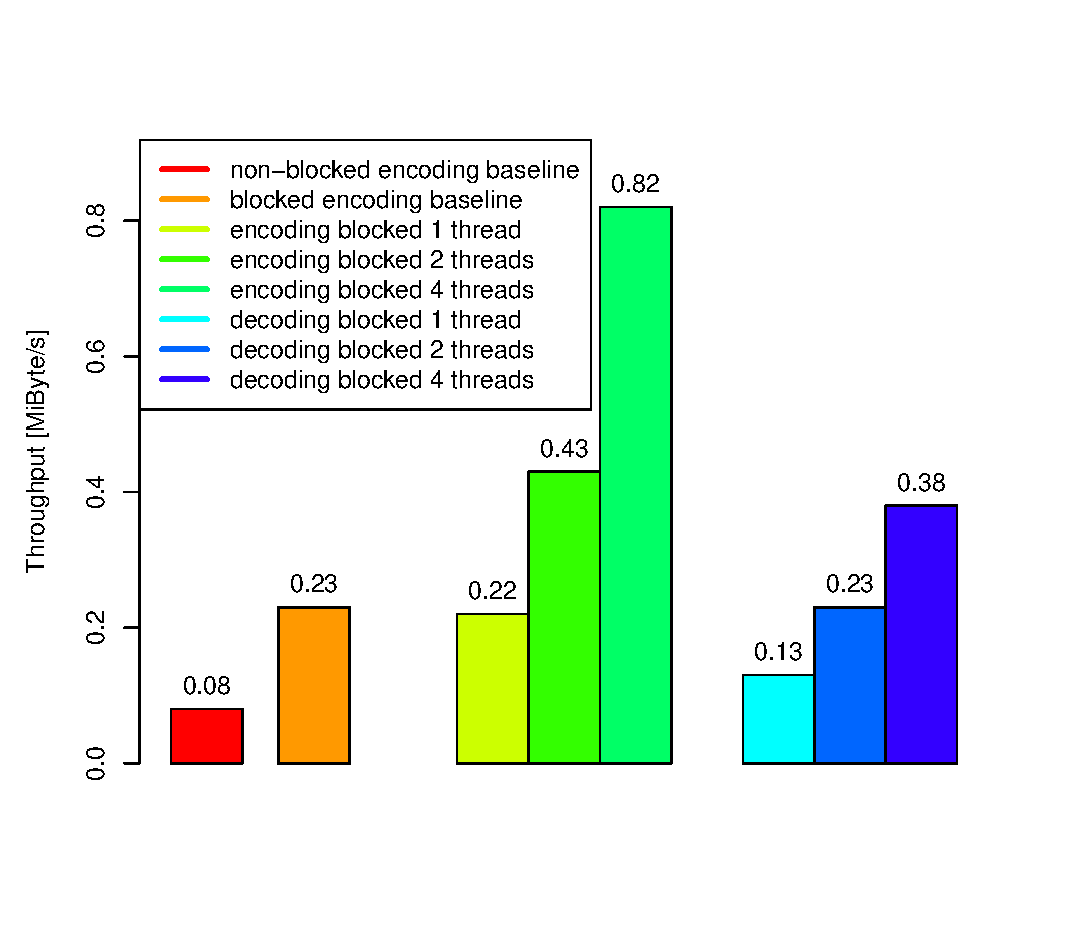
\includegraphics[width=\columnwidth]{images/2015-04-18_encoding_decoding_1024.eps}
\caption{Encoding and Decoding performance for g = 1024}
\label{enc_dec1024}
\end{figure}

\begin{figure}[ht!]
\centering
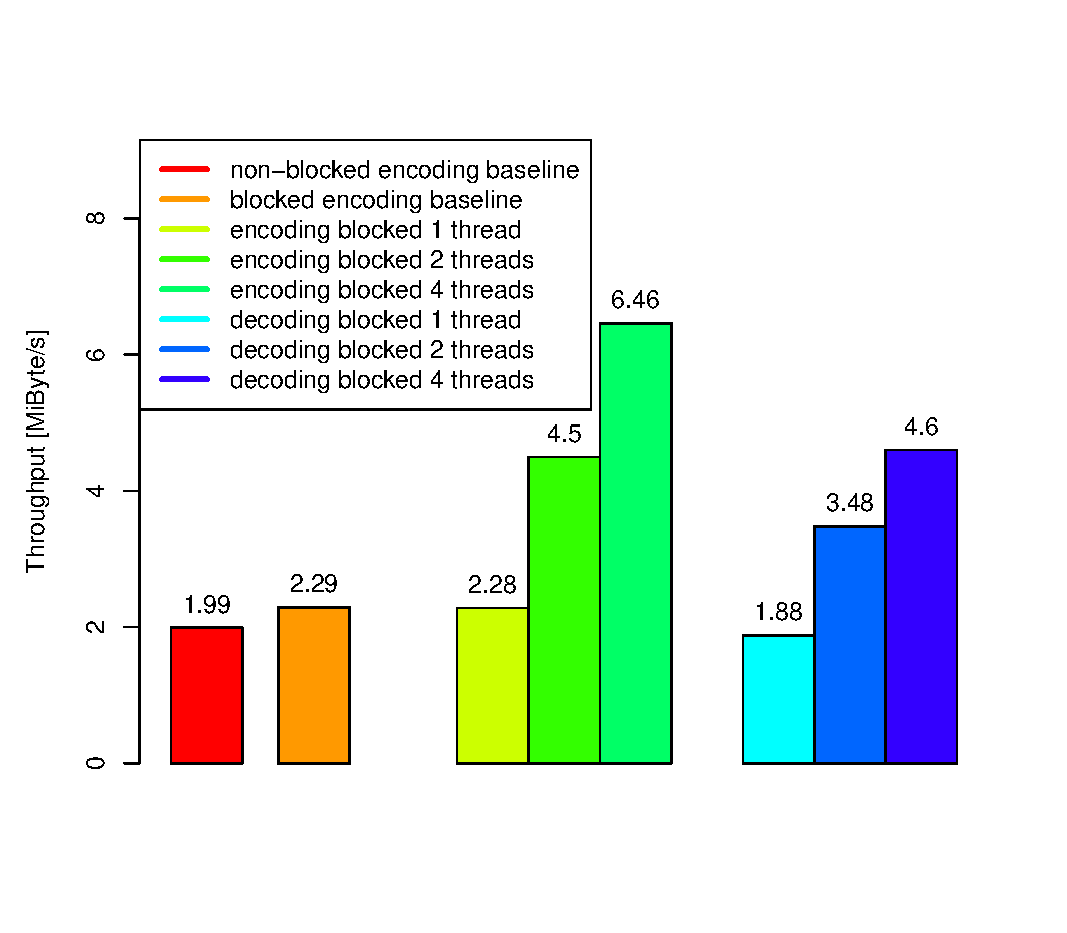
\includegraphics[width=\columnwidth]{images/2015-04-18_encoding_decoding_128.eps}
\caption{Encoding and Decoding performance for g = 128}
\label{enc_dec128}
\end{figure}

\begin{figure}[ht!]
\centering
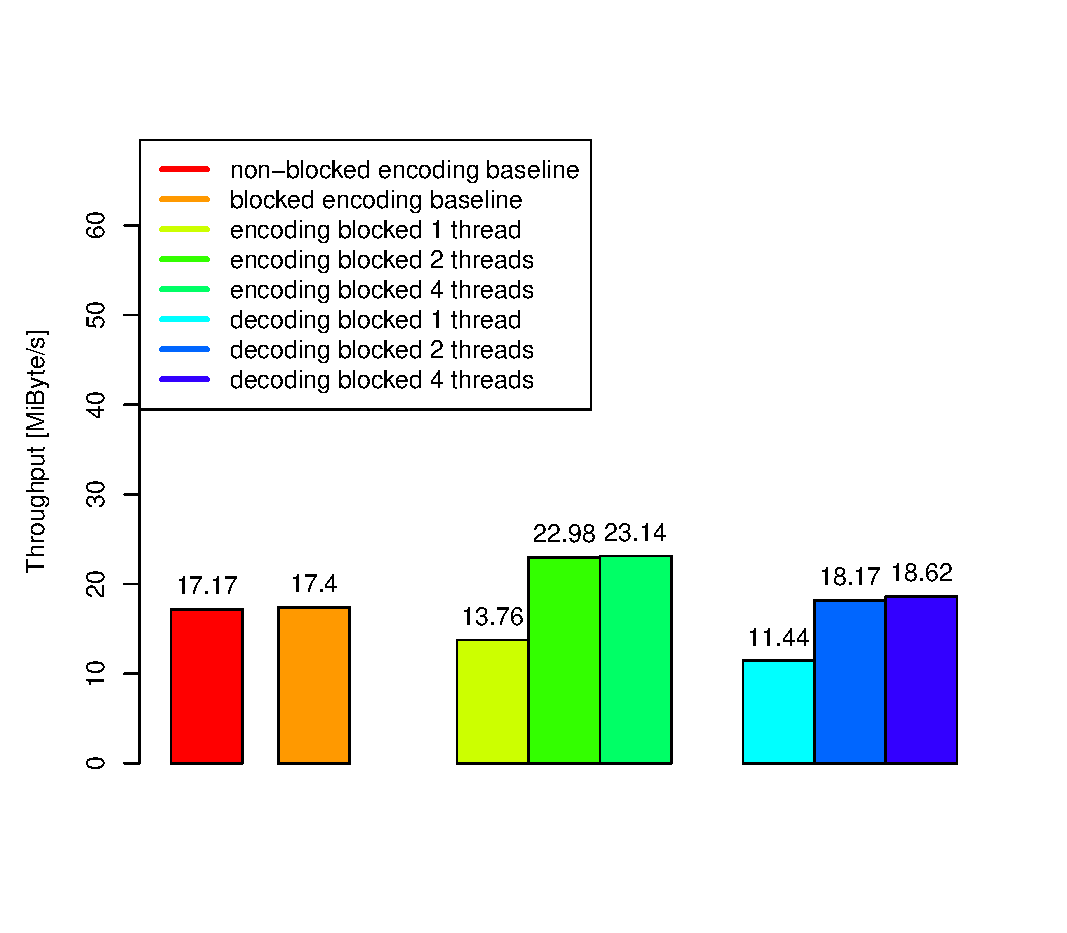
\includegraphics[width=\columnwidth]{images/2015-04-18_encoding_decoding_16.eps}
\caption{Encoding and Decoding performance for g = 16}
\label{enc_dec16}
\end{figure}



\paragraph{Comparison of the load of matrix multiplications and inversions}

\begin{table}[H]
\center
\caption{Multiplication and inversion run-times for different generation sizes with 1 thread}
\begin{tabular}{|r|r|r|r|}
\hline
g & multiplication (ms) & inversion (ms) & ratio \\
\hline
\hline

	16 & 1.703  & 0.345 & 4.9 \\
\hline
	32 & 6.573  & 0.914 & 7.2 \\
\hline
	64 & 21.341  & 3.479 & 6.1 \\
\hline
	128 & 82.326  & 17.411 & 4.7 \\
\hline
	256 & 336.398  & 106.861 & 3.1 \\
\hline
	512 & 1548.750  & 659.469 & 2.3 \\
\hline
	1024 & 6730.380  & 5166.920 & 1.3 \\
\hline
\end{tabular}
\vspace{0.2cm}
\label{runtimes}
\end{table}
